% тут сейчас будут очевидные коментарии
\documentclass[12pt,a4paper]{article}
\usepackage[utf8]{inputenc}		% кодировка утф8
\usepackage[T2A]{fontenc}
\usepackage[russian]{babel}		% локализация
\usepackage{misccorr}			% пакет с дополнительными настройками для соответствия правилам отечественной полиграфии (не знаю, нужен ли, тупо скопипастил)
\usepackage{color}
\usepackage{graphicx}			% чтоб картинки вставлять
\usepackage{amsmath}		    % для формул
\usepackage{amsfonts}
\usepackage{amssymb}
\usepackage{listingsutf8}
\lstset{
extendedchars=\true,            % для вставок кода
inputencoding=utf8,
keepspaces=true}
\usepackage{hyperref}           % оформление ссылок
\usepackage{blindtext}
\usepackage{underscore}         % отдельный пакет для нижнего подчеркивания
%\usepackage[obeyspaces]{url}   % для путей и ссылок
%\UseRawInputEncoding

\graphicspath{ {pic} }       % путь до картинок

%\color[named]{BrickRed}
%\pagecolor[named]{Green}

\begin{document}

\begin{titlepage}
\title{Разработка USB устройства ввода в Linux}
%\thanks{Version 1.0}
\author{Михаил Белкин}
\maketitle
\end{titlepage}

\tableofcontents
\newpage

\section{Введение}
    USB достаточно свежая технология (USB 1.1 - 1998г., USB 2.0 - 2000).
    Задумывалась как универсальная шина для компьютерной периферии.
    И в реальности так оно и оказалось, почти все устройства, даже те что
    раньше были исключительно встроенными теперь можно купить и в USB варианте,
    например, сетевую карту или звуковую карту. Да и вообще на сегодняшний
    день сложнее найти клавиатуру без USB разъема, чем с ним, хотя для
    клавиатур и мышек когда то задумывался отдельный стандартный разъем.
    Я же остановлюсь на чем попроще и соберу геймпад. В общем USB вытеснил
    практически все, его разъем даже больше запомнился как
    стандартный разъем питания на 5В, чем коаксиальный разъем.\\
    К сожалению, я использую всего лишь USB 2.0. В то время, как на данный момент
    уже вышла четвертая версия, чьи скорости превышают SATA в былые времена
    (40 Гбит/с). Но не стоит так сильно беспокоиться, ведь разъёмы до третьей
    версии USB обратно совместимы. Также нельзя не упомянуть и о существовании
    беспроводного USB, которого я практически нигде не видел, но рано или поздно
    мы попробуем и эту технологию.\\
    А данная статья, в отличии от остальных рассматривает процесс разработки
    всесторонне. Также нужно сказать что я не ставил цели написания
    подробной документации на все те программы, которые я использовал. Их вы
    можете найти по ссылкам в списке литературы, в данной статье только
    комментарии к коду. Ниже представлен внешний вид разработанной печатной
    платы устройства и само устройство.\\
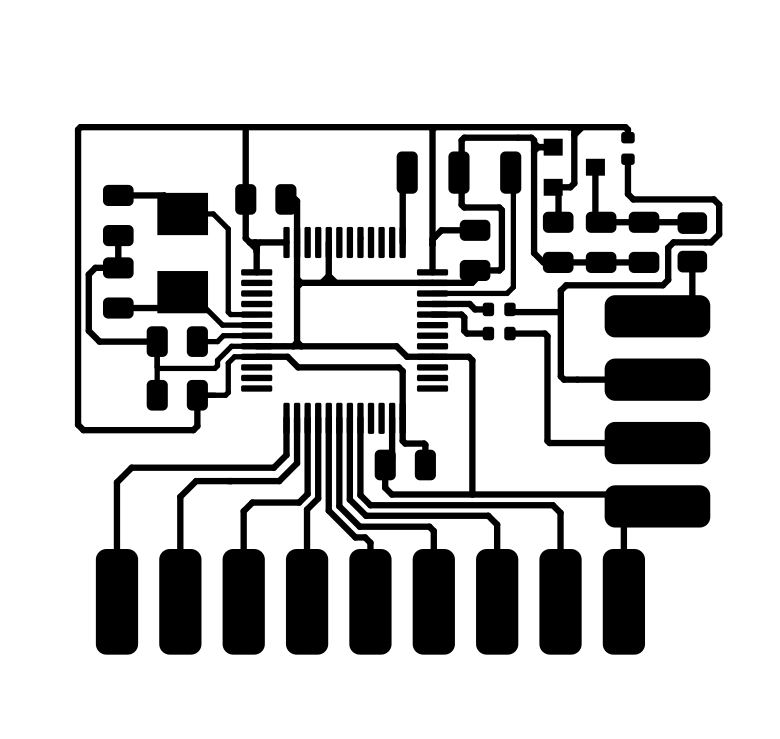
\includegraphics[width=7cm]{pcb.jpg}
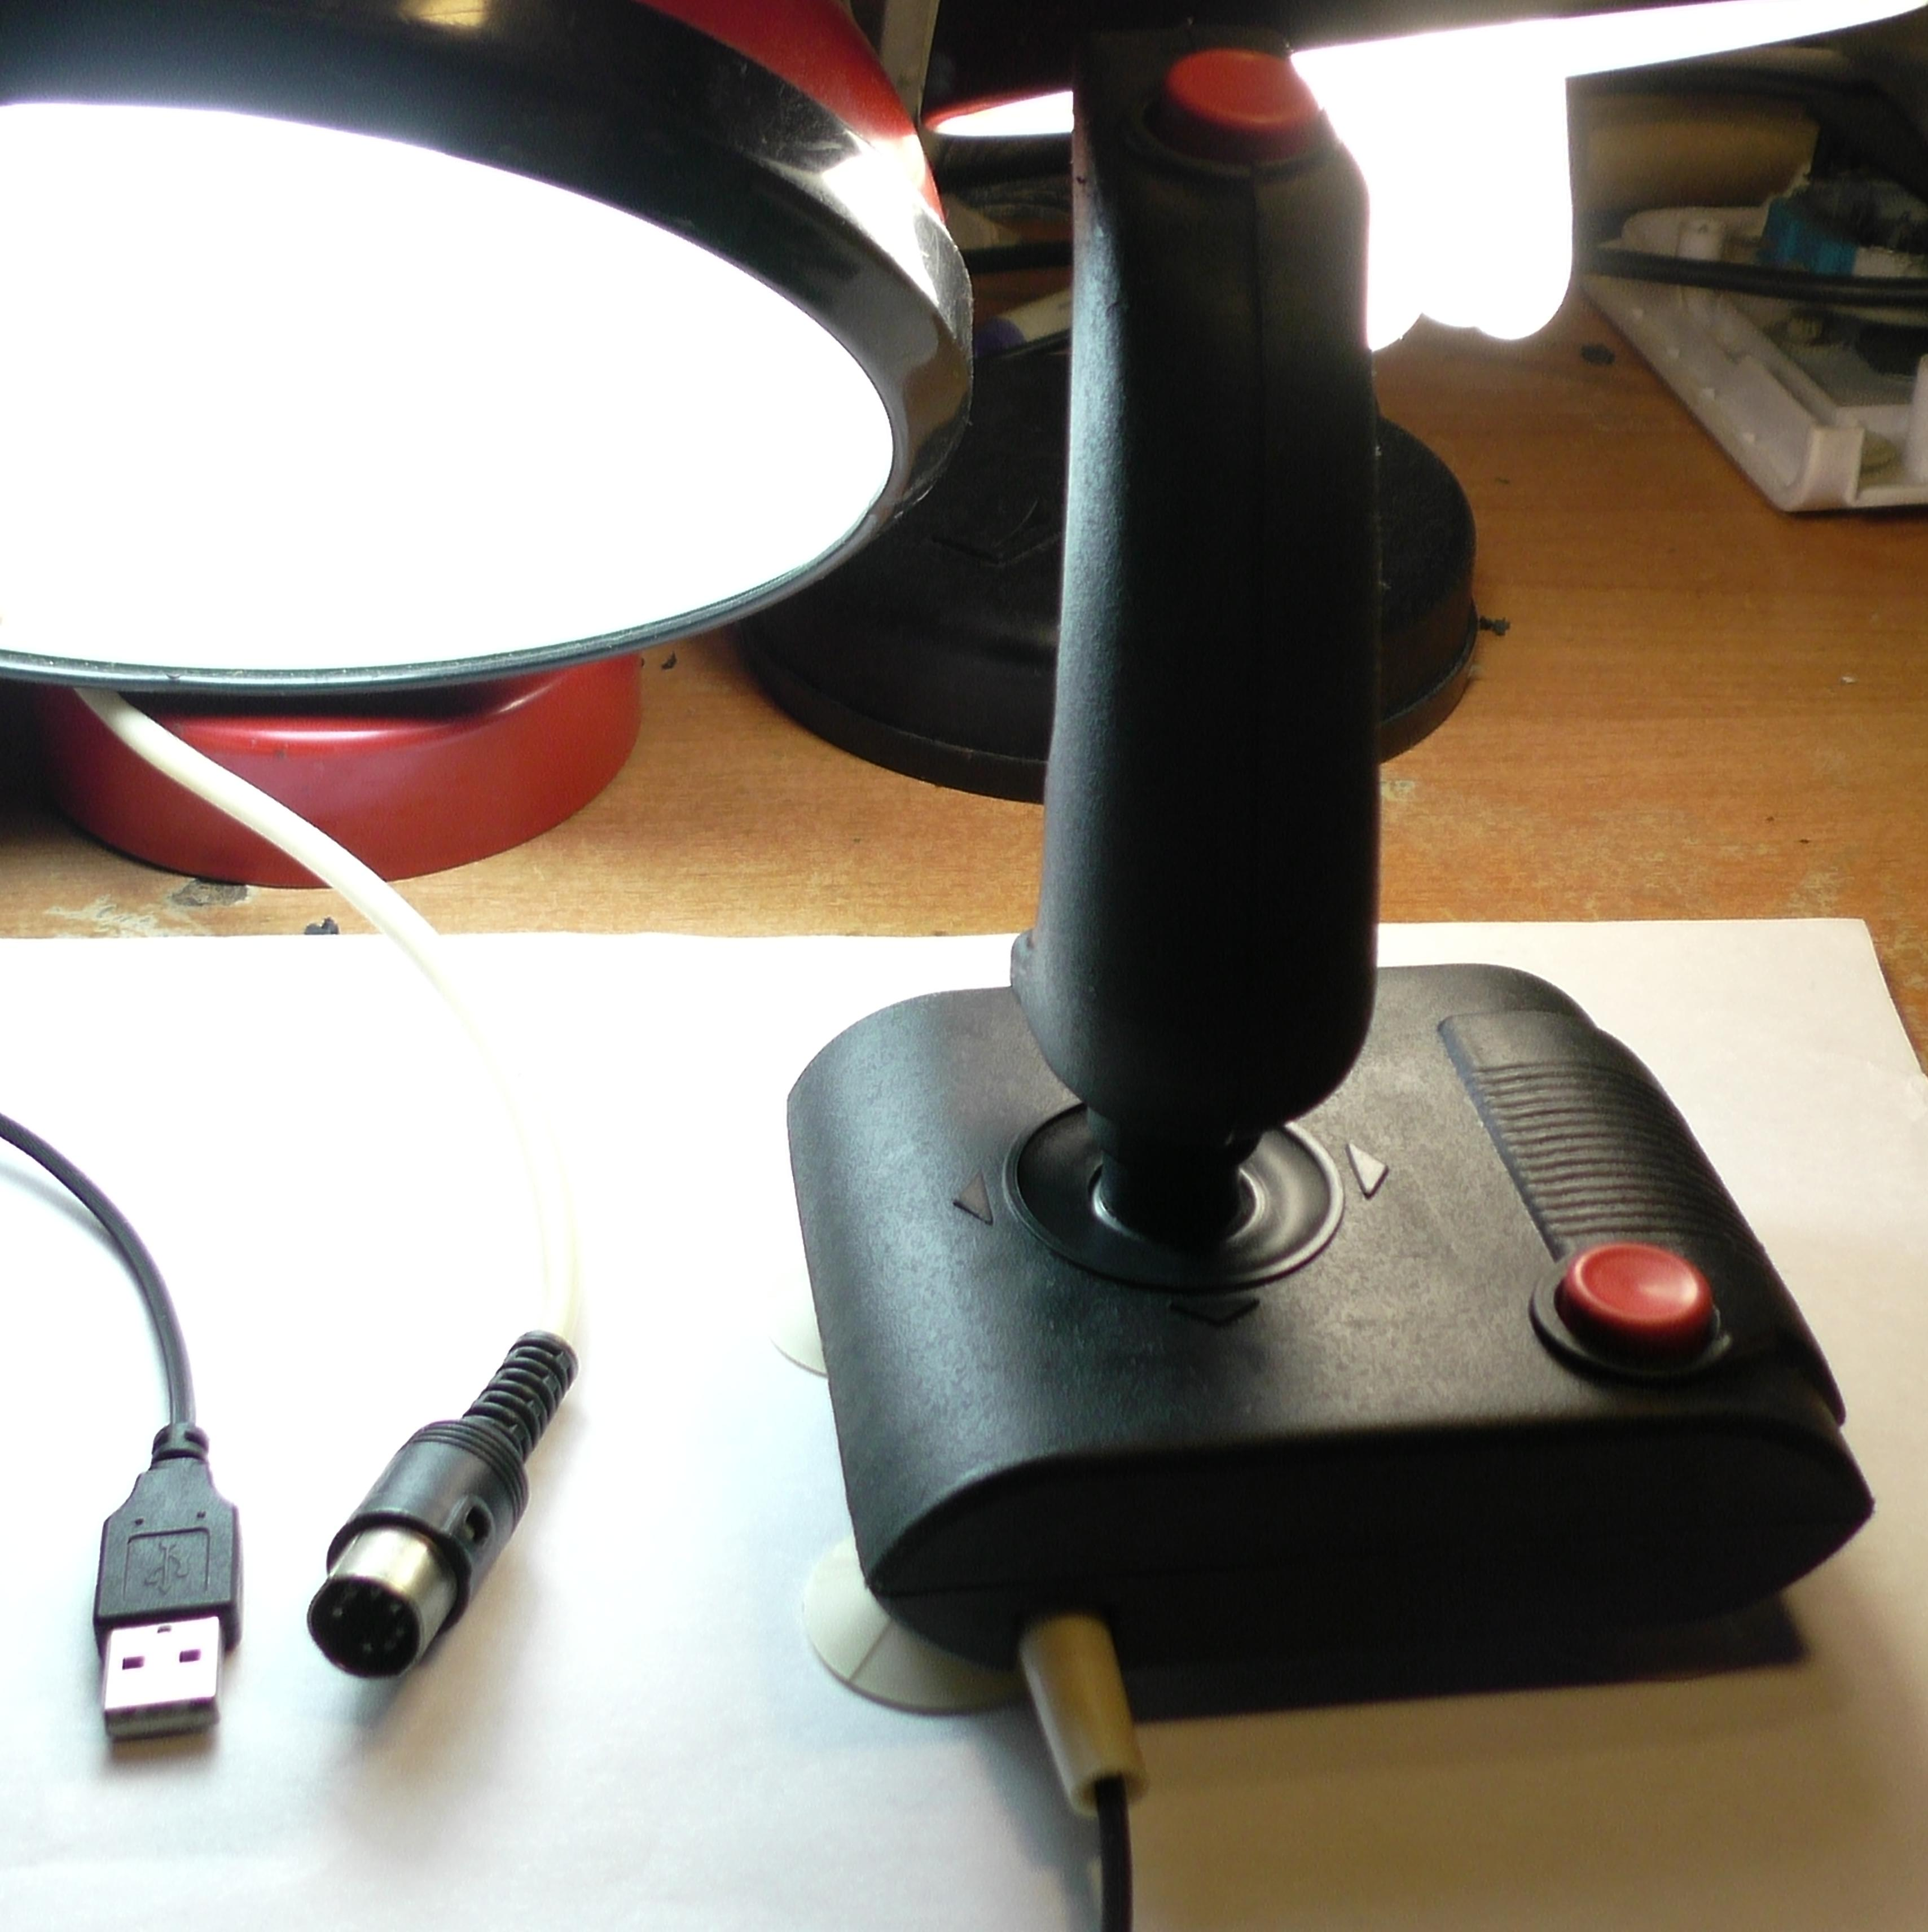
\includegraphics[width=7cm]{gamepad.jpg}\\

\newpage

\section{Схемотехника.}
\subsection{Выбор редактора схем.}
    Разработка схемы производится в KiCAD, это очень легковесный и компактный
    opensource редактор. Но при этом, несмотря на его внешнюю простоту, редактор
    как будто бы кричит нам "Я ничем не хуже чем этот ваш Altium и уж тем более
    Eagle". Поддерживается редактирование многослойных плат, так же используется
    профессиональный подход, при котором схема устройства и печатная плата
    редактируются отдельно. Так же он очень нетребователен к ресурсам
    компьютера.\\
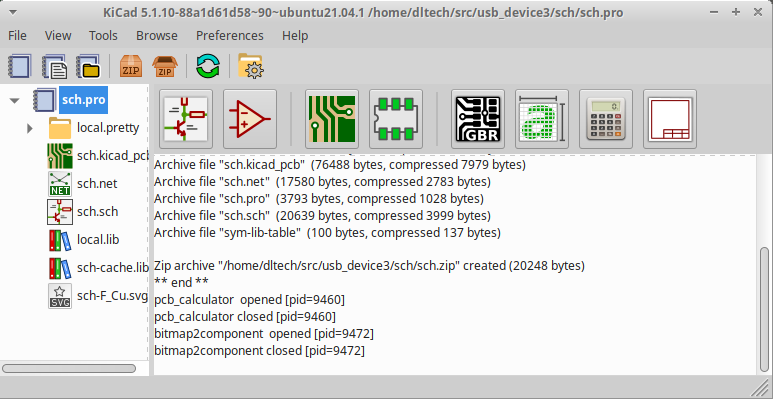
\includegraphics[width=10cm]{kicad1.png}\\
    К редактору имеется собственная библиотека компонентов, которая включает в
    себя компоненты всех популярных производителей, всякие там ST, Ti, можете
    даже не искать. Но если вы принесли
    с китайского базара какую то экзотику, компонент придется разработать
    самостоятельно.\\
    Вывод шаблона печатной платы возможен во всех удобный форматах, включая pdf.
    Так же и Gerber и векторный svg, последнее очень удобно для печати шаблона
    на принтере. Единственное неудобство это не возможность сразу выводить схему
    в растровом формате, приходится самостоятельно конвертировать из svg.\\
    Логично предположить, что данный редактор используется в очень крутых
    проектах. Таких как rusEFI - универсальное ЭБУ для автомобилей, или
    olinuxino - открытый аналог малинки на дешевом китайском чипе от allwinner
    с кучей выведеннных портов на шилд.\\
    В следующем разделе подробно рассказано об скачивании и установке редактора.
    А скачав и установив его вы можете ознакомится со схемой и платой моего
    геймпада, который находится в
    \href{https://github.com/dltech/usb_device3/tree/main/sch}{папке проекта}.\\

\subsection{Установка редактора и библиотек.}
\subsubsection{Установка редактора}
    Установка редактора в Ubuntu Linux производится очень просто, имеется
    отдельный ppa репозиторий с последней стабильной версией. В то время как
    наиболее полный набор библиотек компонентов можно скачать с гитлаба.\\
    Набор команд для установки KiCAD:
\lstset{language=bash}           % Задаем язык исходного кода
\begin{lstlisting}
sudo add-apt-repository --yes ppa:kicad/kicad-5.1-releases
sudo apt update
sudo apt install --install-recommends kicad
\end{lstlisting}
\subsubsection{Установка библиотек}
    KiCAD и библиотеки ужасное сочетание. Те что в репозитории по умолчанию не
    самые полные, актуальное состояние, как всегда, отражает git проекта.
    Безусловно, их можно скачать и добавить в местном проекте, но вот на
    на еще одном компьютере, как всегда, будут проблемы. То есть универсального
    решения попросту нет. Ведь и самое главное что для каждого проекта
     символы то он кеширует, а вот футпринты почему то не хочет.
    Тем не менее, попытаемся написать инструкцию по добавлению библиотек с git.\\
    Итак, до зимы 2020 года библиотеки базировались на гитхабе, сейчас переехали
    на гитлаб. И если у футпринтов формат не поменялся, то символы теперь уже
    адаптированы под еще не релизный шестой кикад. Поэтому символы качаем
    зимние, футпринты сегодняшние. Надеюсь устанавливать git вы умеете и про
    команду git clone вы тоже знаете.
    Вот ссылки на репозитории с библиотеками компонентов KiCAD:\\
    \url{https://github.com/kicad/libraries/kicad-symbols}\\
    \url{https://gitlab.com/kicad/libraries/kicad-footprints}\\
    \url{https://gitlab.com/kicad/libraries/kicad-packages3D}\\
    Скопируйте их все куда нибудь, что бы не мешались, например:
\begin{lstlisting}
cd ~/src/kicad
git clone repo.git
\end{lstlisting}
    Теперь, что бы поставить новые библиотеки так, что бы не мешались старые
    нужно удалить все содержимое папки ~/.config/kicad. При том условии, что
    кикад успел её создать. Дальше заменим пути
    до стандартных библиотек путями на новые. Глобальные пути редактируются
    через контекстное меню. Вкладка Preferenses->Configure Paths...
    Заменяем пути в переменных KICAD\_SYMBOL\_DIR, KISYSMOD и KISYS3DMOD на пути
    до репозиториев kicad-symbols, kicad-footprints и kicad-packages3D, скачанные
    ранее.\\
    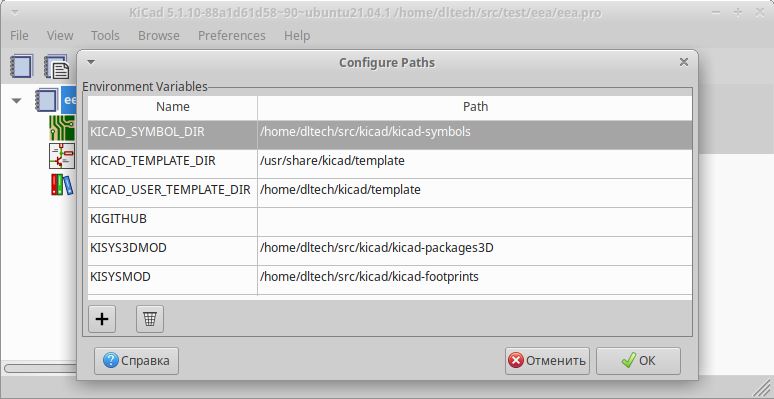
\includegraphics[width=10cm]{kipath.png}\\
    А потом обновляем таблицы компонентов. При первом открытии вкладки
    Preferenses->Manage Symbol Libraries... он должен предложить меню, в
    котором можно выбрать добавление уже существующей таблицы (средний пункт),
    по кнопке ниже
    выбираем путь до файла ~/src/kicad/kicad-symbols/sym-lib-table. Для
    футпринтов аналогично: Preferenses->Manage Footprint Libraries...,
    ~/src/kicad/kicad-symbols/fp-lib-table.\\
    Вот теперь вы можете создавать новые проекты и открывать существующие, имея
    самую полную библиотеку компонентов.
\subsection{Выбор элементной базы.}
\subsubsection{Микроконтроллер}
    Для наиболее аккуратной реализации нужен современный микроконтроллер (МК) с
    полноценным аппаратным USB. Совершенно понятно, что таким микроконтроллером
    окажетcя STM32F103C8T6. Мощное ядро ARM Cortex-M3 с их фирменным вложенным
    векторным контроллером прерываний (NVIC) позволит с легкостью справиться с любой
    задачей. А с такой простой как USB геймпад уж тем более. На борту имеется
    64 килобайта FLASH и 20 килобайт SRAM. И этого настолько много, что можно
    вовсе не думать об оптимизации. Теперь о стоимости, когда то я покупал такой
    за 60 рублей, сейчас цена приблизилась к 200, что по прежнему сравнимо по
    стоимости с остальными морально устаревшими микроконтроллерами. Так же в
    пользу данного микроконтроллера говорит наличие подробной
    документации. О том, почему именно F103, тут все просто, это самый дешевый
    МК с USB из тех что может предложить компания ST microelectronics. Продолжу
    перечислять его преимущества:
\begin{itemize}
    \item Очевидно, 72 мегагерца на 32 разряда.
    \item Гибкая система тактирования, позволяющая отключать всю периферию
    для экономии батарейки.
    \item Поддержка интерфейса SWD и JTAG (прошивка по трем проводам).
    \item А также возможность установки бутлоадеров, один из которых позволяет
    обновлять прошивку по USB (поддержка протокола DFU).
    \item Прерывание, АЦП, выход таймера чуть ли не на каждом порте ввода вывода,
     что упрощает разводку ПП.
    \item DMA (direct memory acсess), по задумке должен упрощать работу с
    периферией, но на практике редко пригождается.
    \item Три 16 битных навороченных таймера счетчика.
    \item Возможность настройки таймеров как для аппаратной поддержки енкодеров,
    так и для различных шим режимов для шаговых двигателей.
    \item Часы реального времени, которые считают даже год.
    \item 2 АЦП со встроенным калиброванным источником опорного напряжения,
    и минимальным временем измерения в 1 мкс.
    \item А также встроенный датчик температуры.
    \item Много прочей стандартной периферии МК (SPI, $I^2C$, CAN, UART)
\end{itemize}

\subsubsection{Стабилизатор}
    В шине USB, как известно, 5В, а номинальное напряжение питания МК 3.3В.
    Поэтому необходим понижающий стабилизатор напряжения. Я рассматривал три
    марки стабилизаторов. Они приведены в таблице ниже:
\begin{center}
  \begin{tabular}{ | l | l | l | l | l | }
    \hline
    стаб & $U_{in max}$ & корпус & производитель & особенности \\ \hline
    L78L33 & 30 & SOT-89 & ST microelectronics &  \\ \hline
    AMS1117-3.3 & 15 & SOT-223 & AMS semitech & термозащита \\ \hline
    XC6206-33 & 7 & SOT-23 & TOREX & CMOS \\ \hline
     \end{tabular}
\end{center}
    И если первый давно знаком многим радиолюбителям. То последние два это
    стабилизаторы от китайских производителей, которые появились недавно.
    В целом гораздо больше доверия к старому 78l, как минимум из за его
    большого входного напряжения. К тому же AMS1117 мне
    попадались нерабочими, и очень легко пробивались от скачков напряжения,
    не спасая нагрузку. Но хотелось бы компактней и подешевле, к тому же
    компьютер сам по себе стабильный источник питания. Поэтому я выбрал XC6206.
    Довольно необычный новодел на полевых транзисторах, в то время как другие
    два на биполярных. Его КМОП структура
    улучшила такой параметр, как минимальное падение напряжения, которое
    всего 0,3В против 1,2В у транзисторных. Также в нем имеется встроенная
    защита по току, чип отключает нагрузку, когда ток превышает 200 мА.
    Ниже приведена его структурная схема, на которой видны
    еще и защитные антистатические стабилитроны. А вот защиты от перегрева у
    него не обнаружено, хотя 1117 что то подобное обещали.\\
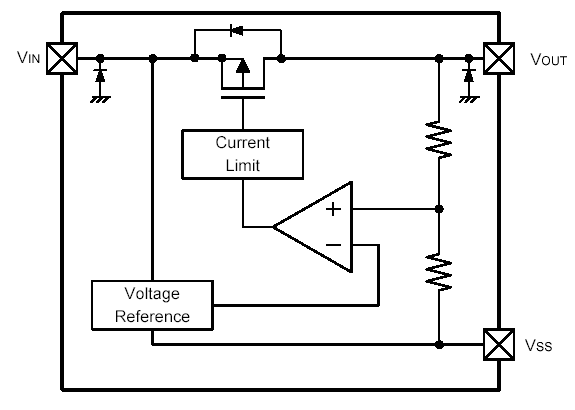
\includegraphics[width=10cm]{6206.png}\\
    Такие стабилизаторы не редкость и часто встречаются на дешевых модулях
    для ардуино.
\subsubsection{Мелочь}
    На форумах можно услышать совет не ставить кварц в целях экономии. Но
    в случае с асинхронной шиной кварц нужен для
    стабильной работы устройства. Микроконтроллер можно настроить на работу от
    самого распространенного кварца на 8мГц. Не удивительно, что на алиэкспресс
    сразу же нашелся не только планарный, но и очень компактный вариант.
    Размером как 1206 чип резистор. \\
    Резисторы размером 0402 я успел заказать заранее. А вот шунтирующие
    конденсаторы пришлось выпаивать с донорских плат, потому они не такие
    компактные, как хотелось бы (0805). \\
    Расчетный ток потребления десятки миллиампер, потому для стабилизации
    питания хватит и чип керамики, благо такая есть даже на 10 мкФ.
    На всякий случай установлю токоограничивающий резистор по питанию.
    Основная его цель обезопасить компьютер от случайного короткого замыкания.
    Хотя в дорогих флешках на его месте можно встретить чип предохранитель.
    Продолжу экономить и на разъемах, попросту ограничусь площадками под
    проводки.

\subsection{Особенность схемотехники USB.}
    На сайте можно скачать целый документ, посвященный вопросу распайки USB
    разъема. Основной вопрос заключается в возможности программного отключения
    устройства от ПК. По стандарту наличие USB устройства на шине определяется
    подтянутым к 3.3В портом DP. В версиях STM32 с USB OTG этот резистор
    встроенный, можно включать и отключать программно. У тех что просто USB
    Device встроенного резистора нету. Поэтому на отладочных платах ST
    устанавливают управление внешним подтягивающим резистором через транзистор,
    подключенный к порту ввода вывода. Моё же устройство будет всегда включено,
    поэтому подтяжка линии DP к питанию будет осуществляться внешним резистором.
    Также важно не забыть про защитные токоограничивающие резисторы, включенные
    последовательно на шинах DM и DP. Провод у меня используется
    готовый от клавиатуры, потому разъем на плате не нужен. Также в дорогих
    устройствах часто можно встретить защитные антистатические стабилитроны на
    шине USB. В моем случае экономим и на них.

\subsection{Схема устройства.}
    А вот и схема целиком, как видите, все шины питания подключены и
    заземлены фильтрующими конденсаторами. Кварц с нагрузочными конденсаторами
    в наличии, так же подтянут к земле и порт сброса. Все как советует официальная документация.
    Кнопки джойстика, как видно, подключены к портам напрямую, т.к. внутри МК
    уже имеются резисторы подтяжки к 3.3В. Плата компактная и помещается внутри
    корпуса, потому дополнительные шунты и защиты не нужны, просто порт.
    Так же не обошлось и без так
    называемого ''грязного хака``, для упрощения трассировки платы один из
    портов ввода-вывода (28 вывод) использован как вывод земли. Но в этом нет ничего плохого,
    ведь порты после сброса находятся в состоянии с высоким входным
    сопротивлением.\\
    Так же на схеме вы можете увидеть и стандартный разъем SWD для прошивки
    и отладки ПО. Ровно как и подключенный на землю вывод BOOT0 означает
    запуск прошивки из основной flash памяти.\\
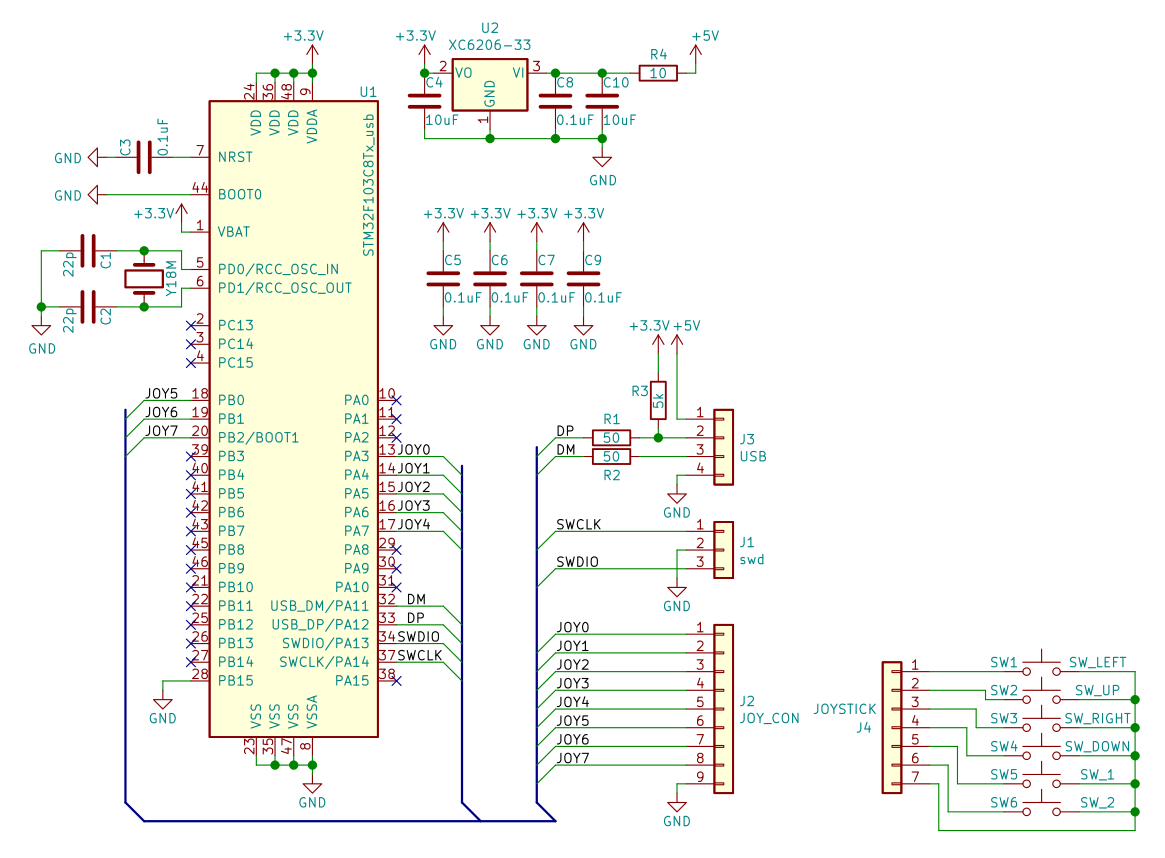
\includegraphics[width=15cm]{sch.png}\\
    А ниже печатная плата с тем самым опасным хаком.\\
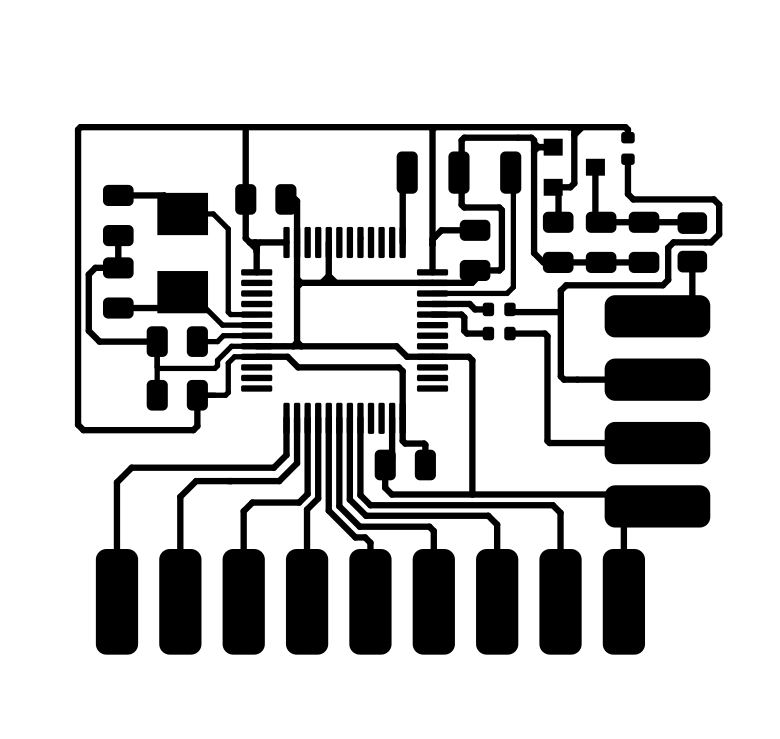
\includegraphics[width=7cm]{pcb.png}

\newpage
\section{Программное обеспечение.}
    Если по началу, когда эти чипы только появились. Выбора способов написания
    ПО для них было немного. Как правило это были коммерческие среды
    среды программирования под Windows, довольно тормозные и
    требовательные продукты. Которые студенты и любители скачивали
    в месте с так называемой таблеткой от жадности. Теперь же выбор
    бесплатных инструментов очень большой. Начиная с официальной среды от
    компании ST, STM32Cube. Которая может не только скачать сама все их
    библиотеки и примеры, но и имеет автоматический конфигуратор периферии (это
    такая штука, которая предлагает настраивать регистры, тыкая мышкой).
    И заканчивая сторонними продуктами, таким как AC6 system workbench.
    И эти новые инструменты, в отличии от старых, уже кроссплатформенные, и
    как это принято говорить на английском, легковесные. Например AC6
    основан на eclipse.
    Так же на гитхабе полно простых устройств, собранных на одном Makefile.
    А ещё сообщество создало полноценную библиотеку libopencm3 с кучей
    примеров.\\
    С прошивальшиком проблем нет, протокол задокументирован, под linux давно уже
    создана st-link utility. Можно даже в отладку, без чего, в случае возни с
    периферией не обойтись. По части периферийных библиотек, доступны как
    варианты от ST так и от проекта libopencm3, тут даже есть выбор.\\
    Но исходя из того, что пример данного устройства довольно простой. Напишем
    весь код полностью самостоятельно. То есть просто представим, что сейчас
    2007 год и мы только что обнаружили новый чип, на который нету ни сред ни
    примеров.\\
    Можно сказать, что программа для ПК и для микроконтроллера ничем не
    отличается. Но на самом деле программы, которые возможно вы писали в школе
    на информатике ориентированы под запуск в операционной системе. И ОС
    значительно упрощает и саму программу и её запуск. В то время
    МК это просто процессор, у которого ничего такого нет. Поэтому вы должны
    самостоятельно описать для него все. Процесс запуска программы, разметку
    памяти, даже компилятор и тот придется запустить самостоятельно, попросить
    у него сохранить прошивку в правильном формате и самостоятельно доставить
    её в микроконтроллер. А также возможно вам придется самостоятельно
    взаимодействовать с ядром.\\
    Весь проект целиком лежит на гитхабе:
    \url{https://github.com/dltech/usb_device3/}

\subsection{Тулчейн.}
    GCC, нисмотря на количество букв Си в этом названии, это не компилятор
    языка Си, а коллекция компиляторов проекта гну. То есть в этой коллекции есть много
    разных компиляторов, в том числе и компилятор языка фортран например.
    Когда то просто скачивание и установка gcc была поводом для отдельного поста.
    Я же отмечу только то, что gcc признает контроллеры на ядре Cortex M3. И
    для этих МК в ubuntu устанавливается вот такой вот командой:
\begin{lstlisting}
apt install gcc-arm-none-eabi libnewlib-arm-none-eabi
apt install gdb-multiarch
apt install build-essential
\end{lstlisting}
    А наши makefile и скрипты прошивки будут их искать потом как
    arm-none-eabi-gcc, arm-none-eabi-objcopy и gdb-multiarch.
    В остальном даже флаги компиляции в случае с данными микроконтроллерами
    ничем особенно не отличаются. Cлово arm в названии пакета, говорит о том, что
    компилятор версии для процессоров arm. А none-eabi означает, что компилятор
    для прошивок, а не для операционных систем.\\
    Все же разберем стандартные для любого проекта флаги:\\
    -ffunction-sections, -fdata-sections - позволит оптимизатору не добавлять в
    прошивку неиспользуемые функции\\
    -Wall -Wextra -Werror -Wconversion -Wundef -Wformat=2 -Wformat-truncation
    -Wdouble-promotion -Wshadow -Wpadded -Wimplicit-function-declaration
    -Wredundant-decls -Wstrict-prototypes -Wmissing-prototypes
    - ворнинги, нужно включить все, какие только возможны,
    понятное дело, что в пяти килобайтах код должен быть вылизан полностью\\
    -fno-common - выдает ошибку если одна и та же глобальная переменная
    объявлена дважды.\\
    -Os - логично, флеша у нас не террабайт, экономим\\
    -mcpu=cortex-m3 -mthumb - обязательно скажем, какой там процессор\\
    -ffreestanding - не подключаем ненужные функции\\
    -ggdb3 - данный параметр нужен для возможности отладки, перед релизом надо
    не забыть его удалить, иначе в прошивке будет много лишних данных.

\subsection{Что нового в CMSIS5.}
    CMSIS это слой абстракции, независимый от производителя. Это не просто
    библиотека, а стандарт взаимодействия с ядром ARM. В библиотеке определены
    главные интерфейсы для инструментов, а также она обеспечивает
    согласованную поддержку устройств. \\
    CMSIS обеспечивает интерфейсы для процессоров и периферии, операционных
    систем реального времени, и компонентов промежуточного программного
    обеспечения. CMSIS включает в себя механизм доставки для устройств, плат,
    и программ, и позволяет комбинировать программные компоненты от разных
    поставщиков. \\
    Важно заметить, что с появлением последней пятой версии она отличается от
    предыдущих, была дополнена и исправлена. Структура проекта CMSIS 5:
\begin{itemize}
    \item Core(M) - стандартизированный API для процессоров Cortex-M
    и периферии. Включает в себя внутренние функции для Cortex-M4/M7/M33/M35P
    SIMD инструкций.
    \item Core(A) - стандартизированный API и базовая система выполнения для
    Cortex-A5/A7/A9 процессоров и периферии
    \item Driver - основные интерфейсы периферийных драйверов для промежуточного
    слоя. Соединяет периферию микроконтроллера со средним слоем что реализует,
    например, стеки связи, файловые системы или графические интерфейсы
    пользователя.
    \item DSP - коллекция библиотек цифровой обработки сигналов с более чем
    60 функциями для различных типов
    данных: целочисленных (дробные форматы q7, q15 и q31) и для чисел с
    плавающей точкой одинарной точности (32 бита). Реализации оптимизированы
    для SIMD наборов инструкций для Cortex-M4/M7/M33/M35P
    \item NN - коллекция ядер эффективной нейронной сети разработанные для
    максимизации производительности и минимизации потребления памяти в
    процессорах Cortex-M
    \item RTOSv1 - основной API для операционных систем реального времени
    вместе с примером реализации основанной на RTX. Это включает компоненты
    программ, которые могут работать в нескольких системах RTOS.
    \item RTOSv2 - расширяет CMSIS-RTOSv1 поддержкой Armv8-M, динамическим
    созданием объектов, поддержку мультиядерных систем, бинарного совместимого
    интерфейса.
    \item SVD - периферийное объявление устройства, которое может быть
    использовано для создания периферийной осведомленности в отладчиках
    заголовочных файлах CMSIS-Core.
    \item DAP - прошивка для блока отладчика которая обеспечивает интерфейс к
    порту системы отладки CoreSight DebugAccess
    \item Zone - определяет методы для описания ресурсов системы и для
    разбиения на разделы этих ресурсов в нескольких проектах и областей
    выполнения.
\end{itemize}
\subsubsection{Скачивание CMSIS5}
    Как ни странно, доступны на гитхабе, как обычно, не будем рисковать
    собой, а получим стабильную версию.
\begin{lstlisting}
cd project_dir
git clone https://github.com/ARM-software/CMSIS_5
\end{lstlisting}

\subsection{Компоновщик.}
    Компоновщик это что входит в состав тулчейна gcc, и занимается эта
    утилита сборкой исполняемого модуля из объектных модулей, полученных в
    результате компиляции.\\
    Устройство довольно простое, почему бы по новой не написать целиком все.
    Итак, не совсем целиком. Если игнорирование официальной библиотеки от
    производителя это уже немного глупо, то игнорировать библиотеки создателей
    процессора просто нельзя. Итак, выбран процессор с ядром ARM Cortex M3,
    значит и будем опираться на файл
    \path{CMSIS/Device/ARM/ARMCM3/Source/GCC/gcc_arm.ld}.\\
    Итак, скрипт компоновщика состоит из:
\begin{enumerate}
    \item разметка памяти
    \item определение входной точки
    \item определения секций
\end{enumerate}
\subsubsection{разметка памяти}
    Компоновщик по умолчанию разрешает разметить всю доступную память, включая
    FLASH и SRAM. Для того, чтобы определить область памяти, которая будет
    использована компоновщиком, и избежать использования каких либо других
    областей памяти, существует команда MEMORY. Она
    обозначает расположение и размер блоков памяти. В шаблоне она уже написана,
    от нас требуется занести адреса в переменные.
    Итак, микроконтроллер STM32F103C8T6 имеет 64кБ FLASH, которые начинаются
    с адреса 0x08000000. Значит
    \textunderscore\textunderscore ROM\textunderscore BASE = 0x08000000,
    \textunderscore\textunderscore ROM\textunderscore SIZE = 0x00010000.
    Оперативная память начинается с адреса
    \textunderscore\textunderscore RAM\textunderscore BASE = 0x20000000, размер 20кБ
    \textunderscore\textunderscore RAM\textunderscore SIZE = 0x00005000.
    Размеры стека и кучи оставим без изменений,
    доверимся примеру.
\subsubsection{точка входа}
    Команда ENTRY используется для определения первой исполняемой инструкции.
    Синткасис команды: ENTRY(symbol), где symbol это переменная, которая обычно
    позже переопределяется в коде. В нашем файле программа стартует с адреса
    сброса - Reset\textunderscore Handler.
\subsubsection{определения секций}
    В скриптах компоновщика переменная точка (.) хранит текущий адрес в памяти,
    в то время как память разделена на секции.
    Команда SECTIONS контролирует то как размечаются input секции в output,
    а также порядок output секций в памяти. Итак, команда SECTION как правило
    используется для определения секции (section definition), которая определяет
    свойства output секций, такие как: ее расположения в памяти, выравнивание,
    содержание, шаблон заполнения, и целевую область памяти. Синтаксис команды
    следующий:
\begin{lstlisting}
SECTIONS {
...
secname start BLOCK(align) (NOLOAD) : AT (ldadr)
    { contents } >region :phdr =fill
...
}
\end{lstlisting}
secname имя секции,\\
start определяет начальный адрес, с которого будет загружаться секция\\
BLOCK(align) выравнивание\\
(NOLOAD) обозначает невозможность загрузки секции во время выполнения программы\\
AT (ldadr) определяет адрес загрузки секции как ldadr\\
>region объявляет секцию как определенную область памяти\\
Служебные слова secname и contents требуются для определения секции, остальные
опциональны.\\
Давайте рассмотрим секцию .text для примера.\\
\begin{lstlisting}
.text :
{
  KEEP(*(.vectors))
  *(.text*)

  KEEP(*(.init))
  KEEP(*(.init))

  /* .ctors */
  *crtbegin.o(.ctors)
  *crtbegin?.o(.ctors)
  *(EXCLUDE_FILE(*crtend?.o *crtend.o) .ctors)
  *(SORT(.ctors.*))
  *(.ctors)

  /* .dtors */
  *crtbegin.o(.dtors)
  *crtbegin?.o(.dtors)
  *(EXCLUDE_FILE(*crtend?.o *crtend.o) .dtors)
  *(SORT(.dtors.*))
  *(.dtors)

  *(.rodata*)

  KEEP(*(.eh_frame*))
} > FLASH
\end{lstlisting}
    .text это имя секции, в секции расположен код. KEEP(*(.vectors)) используется
    для того, чтобы секция векторов прерываний не была оптимизирована (удалена),
    похожий метод применен для секций init, fini, eh\textunderscore frame. Напомним, что переменная
    '.' хранит текущий адрес. Таким образом скрипт извлекает из переменной vectors
    конечный адрес векторов, используя переменную точки, и располагает секцию
    vectors в текущей области памяти.
    Так же располагаются секции dtors и ctors по адресам,
    полученным из crtbegin.o и crtbegin?.o.\\
    Секция ctors это список конструкторов (инициализационных функций),
    который подключает функции, инициализирующие данные в момент запуска программы
    (до запуска функции main).
    dtors устанавливает список деструкторов, которые могут быть вызваны при
    завершении программы.\\
    > FLASH обозначает то, что секция text расположена в области FLASH памяти.\\
    Пролистав и эту унылую теоретическую справку, вы можете догадаться,
    что и здесь со стандартным скриптом компоновщика все в порядке,
    ничего трогать не нужно.
\subsection{startup файл}
    Если коротко, то это такой исходник, который не виден обычным пользователям,
    но именно он вызывает функцию main. Раньше всегда были ассемблерными,
    сегодняшняя версия говорит что он устарел, нужен сишный. Его стандартный
    шаблон находится в:
    \path{CMSIS_5/Device/ARM/ARMCM3/Source/startup_ARMCM3.с}.\\
    Все что нам нужно в нем поменять, так это добавить местных векторов
    прерываний. То есть нужно, что бы компилятор знал, с какого адреса запускать
    то или иное прерывание, если оно произойдет. Позже пользователями в коде
    данные прерывания могут быть переопределены. Важно заметить, что по
    умолчанию для каждого из прерываний в качестве обработчика указан
    бесконечный цикл. Так сделано для того, чтобы контроллер там можно было
    поймать во время отладки. Но важно помнить об этом факте во время
    написания прошивки, т.к. при вызванном и не определенном прерывании
    программа останется в бесконечном цикле. Итак, ориентируясь на Reference
    guide переписываем таблицу прерываний в наш пример. И это все что нужно
    добавить в этот файл для поддержки МК. Т.о. вместо:
\begin{lstlisting}
void Interrupt0_Handler (void) __attribute__ ((weak, alias("Default_Handler")));
void Interrupt1_Handler (void) __attribute__ ((weak, alias("Default_Handler")));
void Interrupt2_Handler (void) __attribute__ ((weak, alias("Default_Handler")));
void Interrupt3_Handler (void) __attribute__ ((weak, alias("Default_Handler")));
\end{lstlisting}
    поучится:
\begin{lstlisting}
void WWDG_Handler (void)__attribute__((weak,alias("Default_Handler")));
void PVD_Handler (void)__attribute__((weak,alias("Default_Handler")));
void TAMPER_Handler (void)__attribute__((weak,alias("Default_Handler")));
void RTC_Handler (void)__attribute__((weak,alias("Default_Handler")));
\end{lstlisting}
    Также и в таблице:
\begin{lstlisting}
WWDG_Handler,   // Window watchdog interrrupt
PVD_Handler,    // PVD through EXTI Line detection interrupt
TAMPER_Handler, // Tamper interrupt
RTC_Handler,    // RTC global interrupt
\end{lstlisting}
    Не забывем внести их же и в заголовочник\\
\path{CMSIS_5/Device/ARM/ARMCM3/Include/ARMCM3.h}:
\begin{lstlisting}
  WWDG_IRQn   = 0
  PVD_IRQn    = 1
  TAMPER_IRQn = 2
  RTC_IRQn    = 3
\end{lstlisting}
    Вот и адаптировали, теперь немного комментариев. Функция Reset\textunderscore handler
    вызывается после сброса микроконтроллера (в момент начального включения
    контроллер так же в состоянии сброса). Она вызывает системную инициализацию
    SystemInit() из файла
    \path{system_ARMCM3.c}, туда позже внесем конфигурацию тактирования. А после
    передает управление функции main, вот и все что делает стартап файлик.
\begin{lstlisting}
__NO_RETURN void Reset_Handler(void)
{
  SystemInit();      /* CMSIS System Initialization */
  __PROGRAM_START(); /* Enter PreMain (C library entry point) */
}
\end{lstlisting}

\subsection{Makefile}
    Внезапно, замороченно навороченный CMSIS не имеет примеров мейков, в
    которых бы заранее были прописаны все его пути. А так стандартный мейкфайл
    на лиж бы запустилось будет выглядеть так:
\begin{lstlisting}
  WWDG_IRQn   = 0
  PVD_IRQn    = 1
  TAMPER_IRQn = 2
  RTC_IRQn    = 3
\end{lstlisting}

\subsection{Тактирование}
    Как изветсно, STM32 микроконтроллер с очень гибкой системой тактирования,
    и самое интересное это, что её можно перестраивать на лету. В случае краха
    неправильных настроек контроллер не остановится, а перейдет на внутренний
    RC генератор на 8 мегагерц. В моей практике дело доходило до того, что
    контроллер запускался от встроенного генератора, поднимал аппаратный SPI,
    по нему конфигурировал периферийный чип на раздачу тактовой. И уже после
    контроллер переключался на это внешнее тактирование. И такой трюк вполне
    успешно работал, экономя немного места на плате.\\
    Итак, вернемся к
    сегодняшнему проекту. Все делители и множители для выбранной конфигурации
    будут выглядеть так:\\
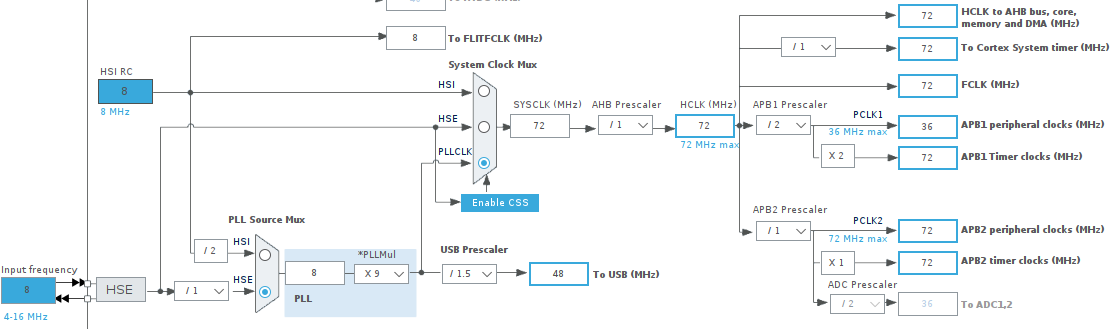
\includegraphics[width=15cm]{tact.png}\\
    Про такой конфиг проще всего сказать что все на максималках. Данная
    диаграмма уже достаточно подробно отражает настройки, все же их перечислю.
    Тактирование от внешнего кварца (HSE) на 8 МГц через PLL, множитель синтезатора 9,
    получаем на выходе синтезатора (PLL) 8*9 = 72 МГц, это и есть sysClk.
    Делитель шины AHB = 1, делитель APB1 = 2, делитель APB2 = 1.
    $F_{AHB}$=72МГц, $F_{APB1}$=36МГц, $F_{APB2}$=72МГц, это максимальные частоты.
    Самое главное не забыть про тактирование USB, для него есть отдельный
    делитель sysClk. Он равен 1.5, т.е. $F_{USB}$=72/1.5= 48МГц, как и должно
    должно быть.\\
    Копировать сюда код получившейся конфигурационной функции не имеет смысла.
    Она интересна разве что циклами ожиданий, пока стабилизируется кварцевый
    генератор и PLL. Потому как контроллер переключается с внутренних 8 МГц на
    PLL только после того, как частота на его выходе стабилизируется.\\
    Еще, выставив максимально возможный sysClk, то есть тактовую процессора,
    важно не забыть указать задержку для считывания flash памяти. Т.к. при
    такой тактовой память окажется медленнее чем проц, и возможно будут
    проблемы. В общем вот этот регистр:\\
    \lstinline{FLASH_ACR |= (uint32_t)FLASH_ACR_LATENCY_2WS;}

\subsection{Структура проекта.}
    Несмотря на кажущуюся простоту, проект все же состоит из 2к строчек кода.
    Потому он очень аккуратно структурирован. Итак, все стандартно, на самом
    нижнем уровне хранятся определения регистров. Также в случае с USB для
    работы с регистрами определены и дополнительные функции (обычно регистры
    поддерживают циклы чтения-записи, и специального обращения не требуют).\\
    На регистры опирается ядро USB,
    оно включает в себя все низкоуровневые функции, а также цикл событий USB,
    реализованный в главном прерывании. Стандартные функции это: функции чтения
    и записи буфера USB, обработчики пакетов, обработка событий сброса, уход в
    спящий режим и возобновление, установщики состояний ендпоинтов, а также
    функция установки адреса и функция инициализации USB.\\
    USB, как известно, работает поверх
    стандартного протокола. Данный протокол реализован в файлах usb\textunderscore st\textunderscore req.c и
    usb\textunderscore hid.c. В первом обязательные стандартные запросы
    контрольного протокола USB, во втором обязательные запросы HID устройств.
     При этом сами обработчики запросов являются внутренними
    функциями, внешней функцией является только функция обработчика запросов,
    которая вызывается ядром. В стандарте определен запрос дескрипторов
    устройства, данные дескрипторы определены в отдельном файле.\\
    Отдельно реализована работа с
    кнопками, которые опрашивают порты ввода вывода. И, наконец, весь проект
    целиком, то есть тот файл, где подключаются и опрос портов и ядро USB
    реализованы в основном файле gamepad.c. По итогу только этот файл и нужно
    подключить для запуска прирложения. Вот и все, по итогу в функции main
    нужно вызвать функцию инициализации gamepad\textunderscore init(), цикл остается пустым,
    т.к. приложение работает полностью на прерываниях.\\
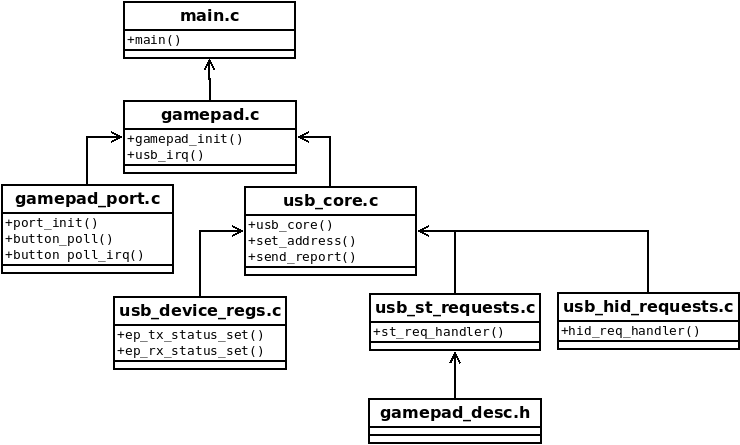
\includegraphics[width=15cm]{proj.png}\\

\subsection{Опрос кнопок.}\label{butt}
    Кнопки в геймпаде обычные, при нажатии контакт кнопки замыкается на землю.
    Потому порты сконфигурированы как входы с включенной подтяжкой к питанию.\\
    По стандарту геймпады и клавиатуры должны отправлять информацию о состоянии
    кнопок в хост. Либо с запрошенной периодичностью в диапазоне
    от 4 до 1020 миллисекунд. Либо, если запрошен период равный нулю, информация
    отправляется только тогда, когда состояние кнопок поменялось.\\
    Итак, для того, что бы получить полную поддержку стандарта, кнопки нужно
    опрашивать постоянно, при этом нужно не забыть про дребезг контактов.
    В моей реализации для опроса состояния кнопок выделен отдельный таймер
    счетчик МК. Счетчик запускает прерывание с периодом в одну миллисекунду.
    В этом прерывании происходит опрос кнопок, если кнопка зафиксирована
    нажатой больше семи раз подряд, программа принимает решение зафиксировать
    это нажатие. Нажатия длительностью менее 7 миллисекунд считаются дребезгом
    контактов и игнорируются.\\
    Это же прерывание тактирует и периодичность отправки данных в хост. То есть
    если cnt больше запрошенного периода (в стандарте обозначен как report duration)
    данные о нажатых кнопках (в стандарте report) отправляются в хост. Где cnt
    счетчик прерываний, срабатывающих каждую миллисекунду. Исключение с
    с отправкой по изменению так же учтено. Вот листинг прерывания:
\lstset{language=c}
\begin{lstlisting}
static int cnt=0;
portPoll();
reportUpdate();
++cnt;
sendReport(gamepadPar.report, &cnt);
\end{lstlisting}
    Сперва опрос портов (portPoll()), потом проверка времени нажатия и запись
    состояния кнопок в переменную report (reportUpdate()), функция отправки
    report. В функцию отправки так же передается внутренний счетчик количества
    вызовов прерываний cnt.

\newpage
\section{USB (универсальная последовательная шина)}
    Интересно заметить, что данный стандарт разработан не IEEE и не ISO, и
    даже не какой нибудь отдельно взятой компанией. Его разработал форум
    компаний, таким образом крупные фирмы решили не городить каждый по своему,
    как это обычно бывает. А просто вместе создали стандарт, который
    бы всех устраивал. К тому же USB Forum организация еще и некоммерческая\\
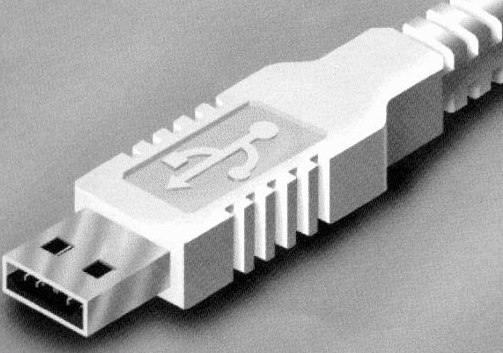
\includegraphics[width=5cm]{plug.png}\\
    Еще один интересный факт, многие из вас помнят шутку про то сколько раз нужно
    перевернуть USB разъем, чтобы его подключить. Тем не менее, стандарт
    учел и эту особенность. Он советует располагать значок USB сверху разъема,
    тогда пользователь может на ощупь определить где верх, и подключить разъем
    не глядя с первого раза.\\
    И как же рассказывать про интерфейс, не упоминая о его скорости.
    В самом лучшем случае, используя USB 2.0 full speed от технологии можно
    добиться 12 Мбит/с. Чего хватит для большинства приложений, например поток
    несжатого аудио занимает всего лишь 1 мегабит. Шина дифференциальная,
    потому вполне работает по длинным проводам.\\
    Данный раздел по сути является переводом официального стандарта, по части
    того, что понадобилось в проекте.
    На всякий случай, приведу таблицу со стандартными типами USB устройств:
\begin{center}
  \begin{tabular}{ | l | l | l | }
    \hline
    00h &	N/A &	Не задано \\ \hline
    01h &	Audio &	Звуковая карта, MIDI \\ \hline
    02h &	Communication Device (CDC)  &	Модем, сетевая карта, COM-порт \\ \hline
    03h &	Human Interface Device (HID) &	Клавиатура, мышь, джойстик \\ \hline
    06h &	Image &	Веб-камера, сканер \\ \hline
    07h &	Printer &	Принтер \\ \hline
    08h &	Mass Storage Device (MSD) &	USB-накопитель, карта памяти, кардридер \\ \hline
    05h &	Physical Interface Device (PID) &	Джойстик с поддержкой Force feedback \\ \hline
    09h &	USB hub &	USB-хаб \\ \hline
    0Ah &	CDC Data &	Сетевая карта, USB-COM \\ \hline
    0Bh &	Smart Card Reader (CCID) &	Считыватель смарт-карт \\ \hline
    0Dh &	Content security &	Биометрический сканер \\ \hline
    0Eh &	Video Device Class &	Веб-камера \\ \hline
    0Fh &	Personal Healthcare &	Индикатор пульса, медицинское оборудование \\ \hline
    DCh &	Diagnostic Device &	USB устройства в отладке \\ \hline
    E0h &	Wireless Controller &	Bluetooth-адаптер \\ \hline
    EFh &	Miscellaneous &	все что не влезло в пр. классы \\ \hline
    FEh &	Application-specific &	режим обновления прошивки (DFU) \\ \hline
  \end{tabular}
\end{center}

\subsection{Краткий обзор технологии USB}\label{1}
    Несмотря на внешнюю простоту (штыревой разъем на четыре провода, куда уж
    проще), у этой технологии есть протокол и четыре уровня абстракции.
    В документациях часто бывают картинки, которые просто нужно вдумчиво
    разглядывать, как будто это ковер. Неторопливо рассматривать каждую
    завитушку причудливого узора. Такая картинка, вернее схема, представлена
    ниже и описывает модель передачи данных USB.\\
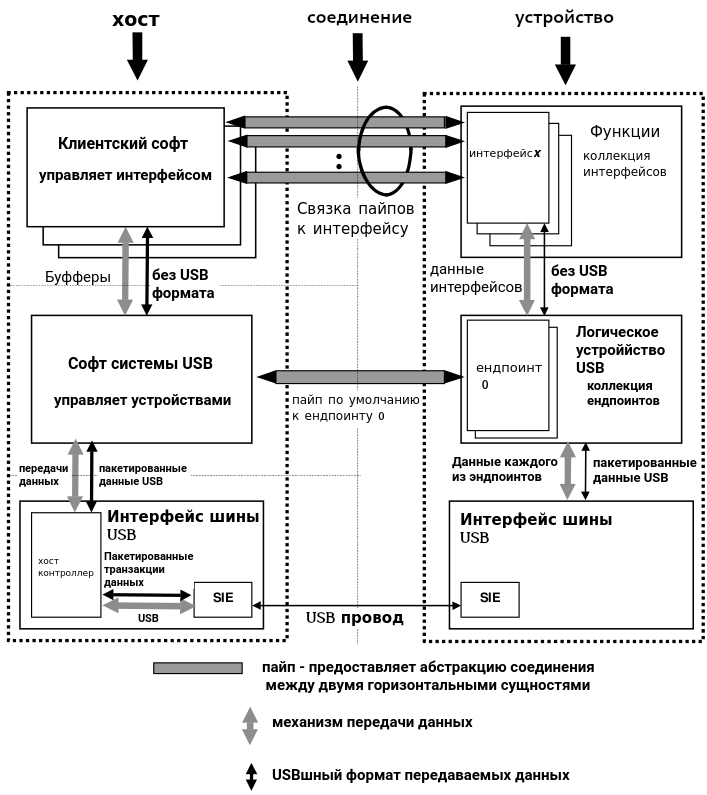
\includegraphics[width=15cm]{protocol.png}\\
    Получив фотокопию внутри себя, пора прочесть пояснения.
    Все что находится на нижних уровнях реализовано аппаратно, то есть давным
    давно отлажено компанией Intel в их IP ядре UTMI, которое и применено
    в выбранном нами чипе. И мы, реализовывая устройство,
    даже и не увидим, что там внутри. Тем не менее, то
    что обозначено на схеме, как SIE (движок последовательного интерфейса)
    скрывает под собой:
\begin{itemize}
    \item электрическую схему интерфейса (драйвер шины)
    \item кодировщик NRZI
    \item обработчик пакетов
\end{itemize}
    В то время, как физически соединение на нижнем уровне представлено
    четырьмя проводами. Положительным и отрицательным проводами дифференциальной
    шины данных (DM и DP), и проводами питания (+5В, GND). \\
    Обмен данными происходит не непрерывно, стандартом предусмотрен протокол, в
    котором осуществляется пакетный обмен данными. Протокол и пакеты это
    тема отдельного раздела стандарта, здесь её рассматривать так же не нужно.
    Все что нам нужно знать, это то, что во всем потоке данных, среди прочих,
     существуют пакеты с данными.
    И прошивка устройства на нижнем уровне работает с их приемом и передачей по
    событию CTR.\\
    Поднимаемся на уровень выше. В середине картинки можно увидеть так
    называемые ендпоинты, дословный перевод конечные точки. Эндпоинт это
    такая фиксированная порция USB устройства, у каждого эндпоинта есть свой
    уникальный буфер и адрес, друг с другом они никак не связаны. А вот поток
    данных между ендпоинтом на компьютере и ендпоинтом в устройстве называется
    пайплайном. Получается, что средний уровень определен обязательным, нулевым
    эндпоинтом, он же еще называется контрольным ендпоинтом. По которому
    осуществляется настройка, определение и начальная конфигурация устройства.\\
    На верхнем уровне находится интерфейсы устройства, то есть уже само
    приложение или приложения (технология USB поддерживает и комбинированные
    устройства). Работают они через все остальные ендпоинты. В моем случае интерфейс
    один, и это интерфейс USB HID
    устройства с двумя кнопками и двумя осями. Работает он поверх одного
    единственного ендпоинта типа Interrupt под номером 1.
    Ендпоинт отправляет пакет с информацией о состоянии кнопок
    с периодичностью в 32 миллисекунды.

\subsection{Периферия USB.}
    А вот и наступила моя любимая возня с регистрами микроконтроллера. Я вам
    наверняка уже говорил, что я собрал свой драйвер под STM, да это так. До
    меня так делала MCD team компании ST и команда libopencm3.

\subsubsection{Включение}
    Как известно, выбранный МК имеет аппаратный USB. Данная реализация аппаратно
    обеспечивает работу двух нижних уровней. Теперь давайте посмотрим,
    что нужно сделать, что бы его хотя бы включить. То есть что бы по шине пошли
    какие нибудь данные.\\
    Как всегда в STM, сперва включаем тактирование, нужно тактирование USB,
    также на всякий случай можно включить и тактирование порта, на котором
    находится USB. Хотя проверено, что настройки портов не влияют на работу
    интерфейса. Итак, нужно выставить биты USBEN и IOPAEN в регистрах шин APB1 и APB2.\\
    Дальше работа с самой периферией непосредственно, необходимо включить USB,
    для этого нужно скинуть биты PDWN, LPMODE, SUSPEND и RESET в контрольном
    регистре USB\_CNTR. Это бит выключения и биты двух спящих режимов.
    А также нужно убедиться в том, что не требуется сброс, и еще нужно сбросить все
    прерывания (занулить регистр USB\_ISTR).\\
    Дальше осторожно, по стандарту USB устройство сперва
    сбрасывается, и только потом разрешается прием и передача данных. Потому
    следующим шагом идет включение прерываний, включая прерывание сброса.
    В моем случае по минимуму: CTR, SUSPEND,
    WAKEUP, RESET. Это событие по приему/передачи пакетов, уход в спячку и
    возвращение обратно и сброс, устанавливаемые в регистре USB\_CNTR.\\
    И уже потом можно выставить нулевой адрес (адрес по умолчанию), за одним
    включив и еще один, я так понял что запасной, бит разрешения приема/передачи
    данных. USB\_DADDR = EF;\\
    Вот и все, на этом можно уже смело считать количество запрашиваемых
    ресетов и ошибок данных в обработчике прерывания USB.
    Как минимум сама по себе периферия уже включена. А вот весь остальной код
    здесь описывать уже не имеет смысла, см. исходник, он короткий и очевидный.

\subsubsection{Буффер USB STM32}
    Для USB в даннном микроконтроллере выделено 512 байт SRAM. Этот раздел памяти
    доступен непосредственно для USB периферии, и для программы пользователя.
    То есть, для отправки пакета программе нужно сложить данные именно в этот
    раздел памяти, а позже периферия их отправит. Так же и с приемом, успешно
    приняв пакет с данными периферия оставит их в этой области, где программе
    их нужно забрать. В документации много говориться о том, что доступ к
    памяти осуществляется на разных частотах (частота интерфейса и процессора
    разные). Но они решили этот вопрос, и там все синхронизировано, можно
    считывать и записывать в любой момент.\\
    Теперь о том, как до нее добраться. Память разбита на слова (16бит), при
    этом указатели у нее 32 битные, потому считывание и запись происходит
    очень весело. Пример записи пакета для отправки:
\lstset{language=c}
\begin{lstlisting}
uint16_t *bufferPtr=(uint16_t*)(USB_ADDR0_TX*2 +USB_CAN_SRAM_BASE_MY);
for(int i=0 ; i<(size/2) ; ++i) {
    *bufferPtr = *input;
    input++;
    bufferPtr += 2;
}
\end{lstlisting}
    То есть здесь видно, что данные в буфер складываются по 16 бит, при этом на
    каждые 16 бит данных, предназначенных для отправки, указатель буффера
    инкрементируется дважды. То есть, в каждых 32х битах хранится по 16 бит,
    причем эти 16 бит младшие.\\
    Но и это еще не все, таблица разметки этой памяти хранится в этом
    же злобном разделе памяти. Но и тут вопрос решается вот такими веселыми макросами,
    заготовленными заранее для каждого эндпоинта:
\begin{lstlisting}
// addresses of endpoint 1
#define USB_ADDR1_TX  MMIO32(USB_CAN_SRAM_BASE_MY+((uint16_t)USB_BTABLE+0x08)*2)
#define USB_COUNT1_TX MMIO32(USB_CAN_SRAM_BASE_MY+((uint16_t)USB_BTABLE+0x0a)*2)
#define USB_ADDR1_RX  MMIO32(USB_CAN_SRAM_BASE_MY+((uint16_t)USB_BTABLE+0x0c)*2)
#define USB_COUNT1_RX MMIO32(USB_CAN_SRAM_BASE_MY+((uint16_t)USB_BTABLE+0x0e)*2)
// addresses of endpoint 2
#define USB_ADDR2_TX  MMIO32(USB_CAN_SRAM_BASE_MY+((uint16_t)USB_BTABLE+0x10)*2)
...
\end{lstlisting}
    Где USB BTABLE это регистр, который хранит смещение, на случай если вы
    захотите разместить таблицу в конце раздела, а не просто в его начале.
    И вот это уже совсем непонятно зачем.\\
    А вот и таблица разметки из моего проекта:\\
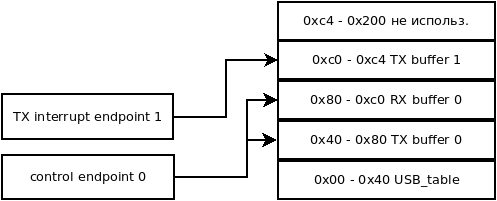
\includegraphics[width=12cm]{table.png}\\


\subsubsection{Ендпоинты}
    Еще раз повторюсь, эндпоинт это порция USB устройства. Эндпоинты бывают
    разных типов, бывают типов isochronous, interrupt и bulk. В моем случае
    нужно всего два эндпоинта двух простейших типов, это двунаправленный
    control эндпоинт и однонаправленный interrupt ендпоинт.\\
    Теперь нужно их инициализировать, во первых, важно заметить, что
    функции инициализации эндпоинтов размещены в функции usbReset(). Т.к.
    прием и передача данных осуществляется после сброса. Сначала нужно
    определить буфферы эндпоинта.\\
    Дальше заполняются данные о типе ендпоинта:
    RX, TX или двунаправленный, или вообще control. Также указывается адрес
    эндпоинта.
    А еще можно попереключать бит DTOG. И все это происходит в регистре
    эндпоинта. Функции работы с битами контроля состояний ендпоинтов описаны
    заранее. Итак, вот
    пример инициализации контрольного эндпоинта:
\lstset{language=c}
\begin{lstlisting}
void usbHidEndpInit()
{
    // инициализация табицы буффера
    USB_BTABLE    = USB_TABLE_ADDR;
    // начальный адрес буффера отправки
    USB_ADDR0_TX  = EP0_TX_START;
    // начальный адрес буффера приема
    USB_ADDR0_RX  = EP0_RX_START;
    // максимальный размер принимаемого пакета
    USB_COUNT0_RX = BL_SIZE_32B | \
    (((EP0_BUFFER_SIZE/32) << NUM_BLOCK_OFFS) & NUM_BLOCK_MASK);
    // ендпоинт с адресом ноль типа control
    USB_EP0R = EP_TYPE_CONTROL | (0 & EA_MASK);
    controlDtogInit(); // обнулить бит DTOG
    epRxStatusSet(0, STAT_RX_VALID); // разрешить прием
    epTxStatusSet(0, STAT_TX_NAK);   // отправка пока не нужна
}
\end{lstlisting}
    После вызова этой функции по нулевому эндпоинту можно принимать и
    отправлять пакеты (control transactions) размером до 64х байт.\\
    Точно так же объявлен и первый ендпоинт. Только он имеет адрес 1 и тип
    interrupt, а еще он типа TX и для него невозможен прием данных, передача возможна. Как
    ни странно, инициализация упакована в функцию usbReportEndpInit().
    После её вызова по нему можно отправлять репорты.
\paragraph{биты DTOG}
    Отдельного внимания заслуживают биты DTOG (data toggle). Они нужны для
    поддержки стабильной непрерывной передачи данных. Есть отдельный на прием, и на
    передачу. Этот бит инвертируется каждую успешную транзакцию и на хосте и на
    устройстве, в случае не совпадения данные игнорируются. Исключение
    составляет control ендпоинт. Для его успешной работы нужно постоянно
    возвращать эти биты в состояние DTOG TX = 1, DTOG RX = 0, под что в моем
    случае отведена отдельная функция controlDtogInit().

\subsubsection{CTRы}
    Данный флаг прерывания включается только по успешному приему данных. По
    логике, оставленной в оригинальном драйвере этот бит должен активироваться
    и после успешной отправки, но этого не происходит. Почему неизвестно, ну и
    ладно, примитивней контроллер - примитивней код, как никак один только
    вызов прерывания откушивает не меньше 11 тактов процессора. Остается только
    легкое беспокойство на тему того, ушли ли вообще отправленные мной данные
    или нет? Да и продолжающий светить бит STAT\_TX\_VALID в регистре ендпоинта
    тоже оставляет меня с чувством незавершенности.\\
    Итак, обрабатываются только RX CTR. В моем случае это события по приему
    новых пакетов конфигурационного пайпа. А его обработчик controlEpRx() по сути только и
    делает, что копирует себе полученный запрос (reqCopy(request)) и передает
    его обработчикам запросов stReqHandler(request) и hidReqHandler(request).
    Вот и вся обработка данных в данном примитивном случае. Логично
    предположить, что обработчики пакетов отвечают по тому же пайплайну.\\
    Хотя один раз TX бит все же срабатывает, он срабатывает после ответа
    подтверждения приема запроса установки адреса. И в этом обработчике
    происходит установка нового адреса. Т.к. по стандарту устройство отвечает
    об успешной обработке команды установки адреса еще по старому адресу, и
    только потом устанавливает новый.\\
    В этой главе добавлю, что раз уж репорт отправляется по interrupt
    ендпоинту. То и функция его отправки вызывается из прерывания считывателя
    нажатий кнопок \ref{butt}.

\subsection{Дескрипоры USB.}\label{158500}
    Во первых их несколько. Во вторых дескрипторы это база данных устройства.
    Как известно,
    USB поддерживает горячее подключение (hot plug). Так вот, после подключения
    устройства к компьютеру, до этого момента не знавшего ничего о нем. Хост
    компьютер может определить его стандартным драйвером за считанные
    миллисекунды (если это linux), или секунды
    (если это windows), и оно будет готово к использованию.\\
    Такие хорошие возможности обеспечивают во многом дескрипторы. Т.к. именно
    в них хранится вся информация об устройстве: его тип, режимы работы,
    скорость, энергопотребление, и то как с ним общаться. И именно дескрипторы
    и запрашиваются во время начальной конфигурации устройства. Так же из-за
    того, что дескрипторы жестко типизированы, занимают они считанные байты.
    Вот существующие типы дескрипторов:
\begin{itemize}
    \item Device - содержит основную информацию об устройстве
    \item Configuration - здесь особенности данного устройства
    \item Interface - у каждого устройства может быть несколько интерфейсов,
    в простейшем случае он один
    \item Endpoint - тут конфигурируется ендпоинт,
    определяются размеры пакетов и частота их передачи, подробнее про ендпоинты
    написано во введении \ref{1}
    \item String - название устройства, которое можно увидеть по команде lsusb,
    хранится в дескрипторах данного типа.
    \item Report - формат репорта
\end{itemize}
    Понятно, что копировать их сюда смысла тоже никакого нет, они лежат в файле
    \path{lib/gamepad_desc.h}. Сюда вынесу описания отдельных переменных из
    дескрипторов, что мне показались интересными.
\subsubsection{Device дескриптор.}
    bLenbght = 18 - длина дескриптора в байтах, стандартно первый параметр для
    любого дескриптора\\
    bDescriptorType = 0x01 - тип дескриптора, так же, стандартно второй
    параметр дескриптора, единица означает device дескриптор\\
    bcdUSB = 0x0200 - 16 битный параметр, обозначающий текущую версию
    спецификации USB, у меня уже USB 2.0.\\
    bDeviceClass = 0x03 - класс устройства, в моем случае USB HID, все
    остальные константы ищите в стандарте.\\
    bMaxPacketSize0 = 0x40 - означает максимально возможный размер пакета в 64
    байта, определенный для нулевого endpoint, в котором и происходит вся
    конфигурация устройства.\\
    idVendor = 0xc410 - для каждого производителя зарегистрирован отдельный ID,
    как правило это производители чипов, я использую STM.\\
    idProduct = 0x0000 - ID продукта, так же регистрируются USB форумом, от
    балды тут ничего написать нельзя, пишем то, что советует datasheet нашего
    чипа.\\
    bcdDevice = 0x0001 - номер релиза устройства по порядку\\
    iManufacter = 0x01 - номер строки содержащей информацию о производителе
    устройства\\
    iProduct = 0x02 - номер строки, с информацией о самом устройстве\\
    iSerialNumber = 0x00 - строка с серийным номером устройства (в моем случае
    не используется)\\
    bNumConfigurations = 0x01 - помните про configuration дескриптор, так вот
    их бывает так же несколько, собери их все, но в моем случае, само собой
    один.
\subsubsection{Configuration дескриптор.}
    TotalLenght = 0x0022 - общий размер почти всех дескрипторов, что есть
    (configuration, interface, endpoint 1, hid)\\
    bNumInterfaces = 0x01 - количество интерфейсов, у меня он просто есть,
    потому что так надо\\
    bConfigurationValue = 0x01 - номер описываемой в дескрипторе конфигурации,
    что бы host мог их выбирать, в случае если их несколько\\
    iConfiguration = 0x00 - и для каждой конфигурации так же можно определить
    строку с описанием\\
    bmAttributes = 0xe0 - стандартные функции устройства, в моем случае сообщим
    только, что устройcтво может может уходить в сон и будиться удаленно и
    запитано от шины USB (бывают и те что запитаны от отдельного блока питания,
    отключаемого по тому же USB)\\
    maxPower = 0x32 максимальный ток, выставим нереальные для моего скромного
    конфига 100 мА
\subsubsection{Interface дескриптор.}
    bNumEndpoints = 0x01 - общее количество endpoint за исключением endpoint 0,
    который по умолчанию\\
    bInterfaceClass = 0x03 - на самом деле о том, что у нас HID устройство,
    нужно говорить тут\\
\subsubsection{Endpoint дескриптор.}
    bEndpointAddress = 0x81 -  endpoint с адресом 1 типа IN (направление данных
    от устройства к хосту)\\
    bMattributes = 0x03 - тип передачи данных по endpoint, в моем случае
    interrupt endpoint, самый простой, не нагруженный\\
    MaxPacketSize = 0x0004 - максимальный размер пакета в 4 байта, что бы
    сообщить о состоянии кнопок нужно немного.\\
    bInterval = 0x20 - интервал запроса данных хостом в 32 мс.
\subsubsection{String дескриптор.}
    В моем случае их три, stringLangId с двумя параметрами:\\
    0x09 English\\
    0x03 U.S. English\\
    И gamepadStringVendor и gamepadStringProduct, хранящие строки zx и joy в
    двухбайтовом юникоде.
\subsubsection{Report дескриптор.}
    usage\_page(Generic Desctop), usage(Game pad) - означают, что стандартное
    устройство ввода для ПК, типа геймпад.\\
    collection(Application) - открывается скобка параметров с основными
    настройками\\
    usage(Pointer), collection(Physical) - вот прямо сейчас точку определим\\
    usage(X), usage(Y) - определим оси x и y\\
    logical\_minimum(-1), logical\_maximum(1) - диапазон от -1 до 1\\
    report\_count(2), report\_size(2), input(Data,Var,Abs) - количество осей и их
    размер, само собой это айтем типа input\\
    usage\_page(Button), usage\_minimum(button1), usage\_maximum(button2) - кнопки,
    две штучки первая и вторая\\
    logical\_minimum(0), logical\_maximum(1) - один бит либо вкл либо выкл\\
    report\_count(2), report\_size(1), input(Data,Var,Abs) - остальная рутина по
    кнопкам\\
    report\_count(2), report\_size(1), input(Const) - выравниваемся до байта\\
    end\_collection(physical), end\_collection(application) - закрываем скобки

\subsection{Стандартный протокол USB.}
    В USB имеется так называемый нулевой конфигурационный ендпоит, он же
    ендпоинт по умолчанию. Он существует для того, чтобы обрабатывать setup
    транзакции (транзакции настройки). В транзакциях данного типа упакованы
    запросы. Среди них есть обязательные, те что определены в основном
    стандарте. И дополнительные, те что определены в стандарте на какой
    то из конкретных типов устройств, например HID реквесты \ref{2}.\\
    Нумерация устройства, запрос дескрипторов, отключение ненужных ендпоинтов
    и включение их обратно. Да и вообще вся служебная работа осуществляется
    через стандартные запросы. Вот их список:
\begin{itemize}
    \item getStatus - запрашивает статус устройства. Двухбайтную переменную,
    которая хранит все динамические параметры устройства.
    \item clearFeature - сбросить функцию. Включает обратно выключенный
    setFeature ендпоинт.
    \item setFeature - установить функцию. Используется для того, чтобы
    увести устройство в спячку, либо выключить какой либо из ендпоинтов.
    Исключая ендпоинт по умолчанию, само собой.
    \item setAddress - установить адрес устройства. Все USB устройства
    стандартно после подключения проходят процесс нумерации.
    \item getDescriptor - запрашивает разные дескрипторы устройства, зависит от
    параметра.
    \item getConfiguration - узнать текущую конфигурацию. На случай, если
    устройство поддерживает несколько
    конфигураций. Если конфиг всего один, все равно должен всегда отвечать, что
    вот тот единственный конфиг и включен.
    \item setConfiguration - установить конфигурацию. Так же должна возвращать
    подтверждение, если первый и единственный конфиг запрошен, иначе ошибку.
    \item getInterface - узнать текущий активный интерфейс. Еще и интерфейсов
    бывает несколько, тут по аналогии.
    \item setInterface - установить интерфейс.
\end{itemize}
    Про протокол запросов можно сказать разве что то, что он ориентирован на
    запрос - ответ, запросы осуществляет хост. В запросе значится в том числе
    и размер возвращаемых в ответе данных. На каждый из запросов отводится
    определенное время на обработку, но можно ответить и раньше. Во всех случаях
    ошибочных запросов
    ендпоинт просто отвечает NAK, то есть заглушенным потоком передачи данных.
\subsubsection{getDescriptor запрос.}
    Данный тип запроса немного интересен тем, что по умолчанию отвечает
    склейкой из configuration, interface, hid и endpoint дескрипторов. При этом
    по отдельным запросам передает любой другой из дескрипторов.
    При чем самое неприятное это
    то, что стандарт говорит просто отбрасывать не поместившиеся в запрашиваемый
    ответ данные, а не отправлять их несколькими пакетами. У меня дескрипторы
    короткие, пакеты по 64 бита, ошибок не вызвало. Также для реализации данной
    функции понадобился конкатенатор дескрипторов descCat(), он же и
    контролирует размер отправляемых данных, что бы был не больше, чем запросили.

\subsection{USB HID}
    HID устройства человеко машинного интерфейса. В это подмножество USB
    устройств укладывается практически все, что взаимодействует с человеком.
    Это и клавиатуры и мышки, и джойстики и рули, и даже костюм виртуальной
    реальности. Также подсветка, управляемая по USB это тоже HID устройство.\\
    Как и говорилось ранее, единственный поток данных который идет из/в USB HID
    это так называемые репорты. Примеры репортов следующие:
    например, клавиатура докладывает о нажатых клавишах,
    либо руль говорит о том, что его повернули на несколько градусов, либо
    компьютер просит поменять цвет подсветки. Репорты чувствительны к времени
    отправки, но поток данных совсем небольшой. Поэтому они передаются через
    interrupt endpoint.\\
    Поток маленький попросту потому, что типы данных и величины определены
    заранее в дескрипторе. А в репорте отправляются сами данные в битовых
    полях. Таким образом, определенная заранее кнопка занимает всего лишь один
    бит в репорте.\\
    Далее рассмотрим формат репорта на примере моего устройства. Его дескриптор
    обсуждался в разделе \ref{158500}.

\subsubsection{HID реквесты}\label{2}
    Для данного типа устройств определены реквесты, дополнительные к основным.
    Их на самом деле много, обязательных всего три, и те, как показала практика
    драйвер так ни разу и не запросил. Вот они:
\begin{itemize}
    \item get report - дополнительный способ запросить репорт.
    \item get idle - считать текущий период отправки репорта.
    \item set idle - установить новый период отправки репорта.
\end{itemize}
    Если основной поток для репорта это interrupt endpoint, то по контрольному
    пайпу тоже можно запрашивать репорт, но такой способ считается
    дополнительным. Также хост может менять периодичность отправки репортов.
    Форматы передаваемых запросов и возвращаемых ими данных можете посмотреть
     в коде, файлы:\\
    \path{https://github.com/dltech/usb_device3/blob/main/lib/usb_hid.c}\\
    \path{https://github.com/dltech/usb_device3/blob/main/lib/usb_hid.h}\\

\newpage
\section{Отладка.}
    Я люблю писать рабочий код с первого раза, потому процесс отладки
    программы я производил очень примитивным способом. Отладчиком gdb через
    терминал, складывая в глобальные переменные все что вызывало сомнения.\\
    Отдельного внимания заслуживает питание устройства. Хорошо, что у меня была еще
    одна плата с таким же процессором, на этот раз отладочная. Контроллер
    в ней запитывался от программатора. Таким образом удавалось не разрывая
    соединение с отладчиком подключать и отключать USB.\\
    Периодически приглядывал за состоянием регистров эндпоинтов USB\_EP0R и
    USB\_EP1R. Смотрел на то, какой присвоился адрес USB\_DADDR, а также
    следил за тем, что происходит в контрольном регистре USB_CNTR.
    Это нужно было что бы понять, правильно ли я взаимодействую с преиферией.\\
    Но самая интересная отладка заключалась в счетчиках прерываний, подсчет
    количества запрошенных сбросов, уходов в спячку, событий wakeup, CTRов, а
    также просто ошибок.\\
    А еще я писал стандартный контрольный протокол опираясь только на
    текст стандарта, и было интересно, насколько его будет понимать стандартный
    драйвер. По итогу я занялся трассировкой стека. Складывал все данные, что
    приходят по контрольному пайплайну в массив. По итогу выяснилось, что нужно быть
    не настолько придирчивым, т.к. один из запросов не совсем строго
    соответствовал стандарту, пришлось удалить несколько перепроверок и
    в целом все заработало. Вот трассировка стека с момента сброса:\\
    DEVICE_GET GET\_DESCRIPTOR DEVICE\_TYP 0 wlen=64 success\\
    DEVICE\_SET SET\_ADDRESS wValue=9 0 wlen=0 success\\
    DEVICE\_GET GET\_DESCRIPTOR DEVICE\_TYP 0 wlen=18 success\\
    DEVICE\_GET GET\_DESCRIPTOR DEVICE\_QUALIFIER_TYP 0 wlen=10 error\\
    DEVICE\_GET GET\_DESCRIPTOR DEVICE\_QUALIFIER_TYP 0 wlen=10 error\\
    DEVICE\_GET GET\_DESCRIPTOR CONFIGURATION\_TYP 0 wlen=9 success\\
    DEVICE\_GET GET\_DESCRIPTOR CONFIGURATION\_TYP 0 wlen=34 success\\
    DEVICE\_GET GET\_DESCRIPTOR STRING\_TYP 0 wlen=255 success\\
    DEVICE\_GET GET\_DESCRIPTOR STRING\_TYP,2 0 wlen=255 success\\
    DEVICE\_GET GET\_DESCRIPTOR STRING\_TYP,1 0 wlen=255 success\\
    DEVICE\_SET SET\_CONFIGURATION wValue=1 0 wlen=0 success\\
    33 GET\_INTERFACE 0 0 wlen=0 success\\
    INTERFACE\_GET GET\_DESCRIPTOR REPORT\_TYP 0 wlen=48 success\\
    Надеюсь о существовании команды print и ее шестнадцатеричном варианте p/x
     в gdb моей аудитории рассказывать не нужно.



%\begin{thebibliography}{9}
%\bibitem{lamport94}
%  Leslie Lamport,
%  Addison Wesley, Massachusetts,
%  2nd edition,
%  1994.
%\end{thebibliography}


\end{document}
